\chapter{SMACK Verification Framework}\label{ch:smackframework}
Developing a full featured software verification tool from end-to-end
can be a daunting task.  Bounded model checking requires several
steps.  First, the input source code must be parsed or compiled.  The
resulting abstract syntax tree (AST) must then be semantically
interpreted, and a model built of underlying program semantics.
Finally, the modeled program must be represented as an SMT query and
passed through an SMT solver.  This imposes a large barrier to entry
for prototyping a new model checking algorithm, or building a
verification tool for a new source language using existing
algorithms. 

The Boogie intermediate verification language (IVL) was designed by
Microsoft Research to alleviate the complexity of modeling new source
languages and implementing new model checking algorithms.  Boogie IVL
separates the task of modeling input program semantics from the task
of bounding and checking modeled programs.  This allows model checking
tools to take Boogie IVL files as input, rather than the input source
language.  Similarly, front-end tools can model the input program
semantics in Boogie IVL rather than being directly integrating with
the model checker.  By providing a clear, distinct interface between
the two tasks, Boogie IVL [allow for modular tool components rather
than end-to-end verification tools]. 

Due to its goal of creating an abstraction between program modeling
and model checking, Boogie IVL has been designed to be a very
low-level modeling language.  It contains support for little more than
a typing system, basic arithmetic and boolean expressions \&
statements, control flow \& procedure calls, and verification
condition specification~\cite{boogie}.  Any more complicated semantics
of the source language must be modeled using the basic set of
primitives available in Boogie IVL. 

Though the low-level nature of Boogie IVL provides the flexibility to
support a large variety of models of computation and source languages,
it requires that models be created to define the semantics of
operations available within the source language and computational
model environments.  As an example, there is no concept of a heap
within Boogie.  Because of this, a memory model must be developed that
accurately models the behavior of the heap.  A rudimentary model of
memory could use a simple, large array of integers to represent the
heap, where each element represents a word of memory, and C pointers
are simply indices into this array. 

[I don't like the phrasing/organization of this next paragraph - I
feel it highlights the Boogie verifier too much, and I don't have much
to say about the Boogie verifier] 

As the goal of Boogie IVL is to modularize model checking verifiers,
it shouldn't be surprising that there are several back-end model
checking tools that support Boogie IVL programs.  The original
back-end for Boogie IVL is a tool called Boogie.  In addition to being
a complete back-end verifier for Boogie IVL programs, it also provides
an API for parsing Boogie IVL and interfacing with SMT solvers.
[Paragraph intro sentence indicates paragraph will be talking about
several verifiers, but only discusses Boogie] 

[Where to put this paragraph?] It should be noted that there exists a
back-end verifier from Microsoft Research named Boogie.  The Boogie
program verifier provides similar functionality to the Corral program
verifier.  Hereafter, ``Boogie'' will refer to BoogiePL unless
otherwise specified. 

[Bad paragraph - gets sloppy in last few sentences]Corral is another
back-end Boogie IVL program verifier, and is a good example of how
Boogie simplifies the implementation of new model checking algorithms.
Corral leverages the Boogie verifier API to implement additional model
checking algorithms, such as the Lal/Reps sequentialization algorithm
[cite this - Reducing Concurrent Analysis Under...].  [... With this
and other algorithms, ] Corral has put considerable effort toward
providing [cutting-edge] support for analyzing concurrent programs.
As such, it was the ideal candidate to use as a back-end verifier for
the pthreads extension of SMACK. 

Though providing state of the art algorithms for checking concurrnt
programs, Corral is similar to the Boogie IVL in that it provides only
low-level support for modeling concurrency.  The Corral program
verifier provides an extension to Boogie IVL that includes a very
basic set of primitives for modeling concurrent programs.  This
extension includes the following calls: 

\begin{itemize}
\item \lstinline|async call| \emph{func}\lstinline|(|\emph{...}\lstinline|)| - Asynchronously calls \emph{func} with the parameter list \emph{'...'}
\item \lstinline|corral_atomic_begin()| - Begins an atomic block
\item \lstinline|corral_atomic_end()| - Ends an atomic block
\item \lstinline|corral_getThreadID()| - Returns the ID of the calling thread.
\item \lstinline|corral_getChildThreadID()| - Returns the ID of the thread most recently spawned in the calling procedure.
\end{itemize}

The behavior prescribed in the pthread specification [cite pthreads
specification] is much more complex than these low-level concurrency
primitives recognized by Corral.  As a result, to provide support for
the more complex pthread API, it is necessary to build a model of the
pthread API behavior using the primitives provided by Corral. 

[Transition from modeling in Boogie to SMACK][major work needed below this point]

Once the behavior of the pthread API has been accurately modeled in
Boogie, the front-end [someadjective] component must be extended to
translate pthread API calls in the input source into the Boogie IVL
model of the pthread calls. 

The SMACK project as a whole is an end-to-end C/C++ program verifier.
At its core, the SMACK executable is essentially a compiler that takes
C/C++ programs and translates them into Boogie IVL~\cite{smack}.   


The SMACK toolchain is depicted in Figure~\ref{fig:SMACKToolchain}.
SMACK as a whole is a front-end for a program verification toolchain
that features the Corral program verifier as its core back-end.  Input
C/C++ programs are given to Clang to compile and link, resulting in an
LLVM bytecode output.  This is then passed to the SMACK executable,
which translates the LLVM bytecode into a Boogie program that models
the behavior of the input C/C++ program.  The resulting Boogie program
is then passed to Corral.  Corral converts the Boogie program into an
SMT query, which is given to the Z3 SMT solver for evaluation. 

SMACK itself is essentially a compiler that takes C/C++ programs and
translates them into Boogie IVL~\cite{smack}.  This converted Boogie
code is then consumed by a static analysis tool that evaluates
verification conditions present in the original source code. 

\begin{figure}[!h]
  \caption{SMACK Toolchain}
  \label{fig:SMACKToolchain}
  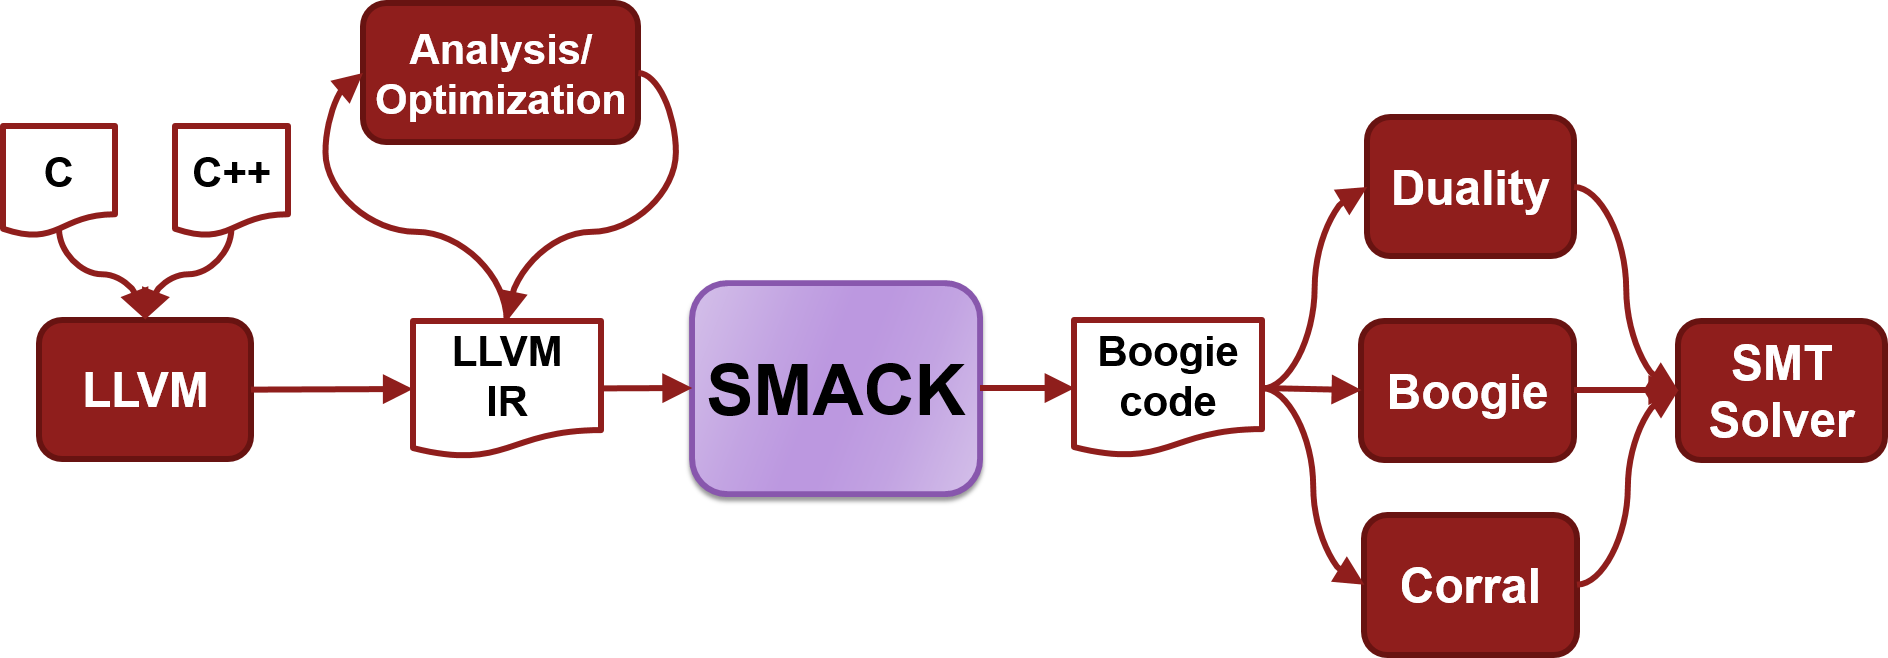
\includegraphics[width=1\textwidth]{SmackToolchain.png} 
\end{figure}


\section{Modeling Environment}\label{sec:modelingenvironment}
[Redo intro]
As described in Chapter~\ref{ch:smackframework}, SMACK consumes LLVM IR
bytecode, builds a model of the input program, and generates a Boogie
IVL model of the input program.  The design of this toolchain leaves
us with several levels at which modeling semantics can be introduced.
At the C level, external library functions that are otherwise
undefined can be given a definition, rather than verifying the whole
original source library. At the SMACK translation level, undefined
functions can be intercepted so SMACK can perform predefined
alterations to the translated Boogie program rather directly being
translated from the LLVM IR representation.  At the translated Boogie
level, additional variables and instructions can be added to model
environmental functionality that is not defined at the C level.
Finally, there can be additional functionality modeled by the Boogie
IVL solver itself. 

To provide some context for the discussion of the modeling process,
I'll briefly introduce Boogie IVL, and then discuss the mechanisms
used for modeling, such as the Corral concurrency primitives and C
level Boogie injection.

\subsection{Boogie IVL}
[Good]
Perhaps the most illustrative way to introduce Boogie IVL may be to
show an input C program and the relevant portions of the Boogie output
that SMACK returns.
\begin{figure}[h]
\centering
\caption{SMACK Translation of C Program}\label{fig:cToBoogie}
\begin{subfigure}[b]{.45\textwidth}
\centering
\caption{Input C Code}\label{fig:cToBoogie_a}
\begin{lstlisting}


void main() {
  int *x, *y;
  x = malloc(sizeof(int));
  y = malloc(sizeof(int));
  *x = 1;
  *y = 2;
  assert(*x == 1);
}
\end{lstlisting}
\end{subfigure}
~
\begin{subfigure}[b]{.45\textwidth}
\centering
\caption{Boogie Code from SMACK}\label{fig:cToBoogie_b}
\begin{lstlisting}[language=boogie]
var $M: [int]int;

procedure main() {
  var $x, $y: int;
  call $x := $malloc(4);
  call $y := $malloc(4);
  $M[$x] := 1;
  $M[$y] := 2;
  assert($M[$x] == 1);
}
\end{lstlisting}
\end{subfigure}
\end{figure}

Figure~\ref{fig:cToBoogie_b} shows a reduced version of the Boogie
code as translated by SMACK from the input source depicted in
Figure~\ref{fig:cToBoogie_a}.  Translating source language programs
into Boogie IVL programs like this provides a common language on which
to perform verification for solvers like Corral, Boogie verifier, and
Duality.  

\subsection{Corral Concurrency Primitives}
[Good]
Corral is a state of the art solver for Boogie IVL programs.  One of
Corral's recent development efforts has been to improve support for
verifying concurrent programs.  To this end, Corral has extended
Boogie IVL, and recognizes five concurrency primitives that are not
part of the base language.  These are [choose whether to list here or
in background]: 

\begin{itemize}
\item \lstinline|async call|
  \emph{func}\lstinline|(|\emph{...}\lstinline|)| -- Asynchronously
  calls \emph{func} with the parameter list \emph{'...'} 
\item \lstinline|corral_atomic_begin()| -- Begins an atomic block
\item \lstinline|corral_atomic_end()| -- Ends an atomic block
\item \lstinline|corral_getThreadID()| -- Returns the ID of the
  calling thread.
\item \lstinline|corral_getChildThreadID()| -- Returns the ID of the
  thread most recently spawned in the calling procedure. 
\end{itemize}

\begin{figure}[h]
\centering
\caption{Corral Concurrency Primitives in Action}
\label{fig:corralprimitives}
\begin{lstlisting}[language=boogie]
var $x: int;

procedure f() 
  modifies $x;
{
  var $tid: int;
  var $tmp: int;
  call $tid := corral_getThreadID();
  call corral_atomic_begin();
  $x := $tid;
  $tmp := $x
  call corral_atomic_end();
  assert($tmp == $tid);
}

procedure main() {
  var $ch1, $ch2: int;
  $x := 0;
  async call f();
  $ch1 := corral_getChildThreadID();
  async call f();
  $ch2 := corral_getChildThreadID();
  assert($x == $ch1 || $x == $ch2);
}
\end{lstlisting}
\end{figure}

Figure~\ref{fig:corralprimitives} demonstrates the usage of each of
these primitives within the context of a complete Boogie program.
This program initializes the global variable \lstinline|$x| as 0, then
makes two asynchronous calls to the function \lstinline|f()| and
records the thread ID of each of the spawned threads of execution.  In
\lstinline|f()|, each of the spawned threads records their thread IDs.
Each thread then starts an atomic block, where it stores its thread ID
to the global \lstinline|$x| and then loads global \lstinline|$x| into
the local \lstinline|$tmp|.  The \lstinline|assert()| in
\lstinline|f()| should always succeed, since \lstinline|$x| is stored
and loaded within an atomic block. 

However, this program contains a bug.  Because there is no barrier
forcing the parent to wait for the child threads to execute, it is
possible that \lstinline|$x| won't be set to the thread ID of either
children by the time \lstinline|assert()| is called in
\lstinline|main|.

It is this additional support for concurrency that warranted selection
of Corral as the solver to target for extending SMACK to support pthreads.

\subsection{C Level Modeling}
[Ok.  Could use another pass or two]
Because there are several layers at which model semantics can be
introduced, SMACK has introduced several special C level functions 
that don't get directly translated into Boogie code, allowing users to
introduce program semantics at the lower levels of the modeling
environment by writing code at the C level.  This allows OS
environment and library models to be completely written as C input
programs, which avoids modifying SMACK's source code directly to
implement such models.

An example of this is \lstinline|malloc|.  Rather than having SMACK
itself append a memory model and \lstinline|malloc| definition to each
translated Boogie program, these semantics are instead defined in a
header file that gets included from each input program.  Clang
compiles this included header file, so when SMACK begins translation,
the memory model and \lstinline|malloc| are present in the AST,
leaving SMACK with only the responsibility of translating the LLVM IR.

There are several C level functions that SMACK treats specially when
seen in the LLVM IR AST.  Upon seeing these, SMACK performs special
transformations to the Boogie translation, rather than translating the
function calls as is.  Two of these functions were particularly
important for the pthread extension to SMACK. 


\begin{itemize}
\item \lstinline|__SMACK_code(char* format, ...)| -- Injects the
  string \lstinline|format| in the Boogie code.
\item \lstinline|__SMACK_top_decl(char* format, ...)| -- Inserts the
  string \lstinline|format| as a global declaration 
\end{itemize}

\begin{figure}[h]
\centering
\caption{Injecting Boogie Code from C}\label{fig:cinjToBoogie}
\begin{subfigure}[b]{1\textwidth}
\centering
\caption{Boogie Injecting C Code}\label{fig:cinjToBoogie_a}
\begin{lstlisting}
void main() {
  __SMACK_top_decl("var $globalVar: int;");
  int *x;
  x = malloc(sizeof(int));
  *x = 1;
  __SMACK_code("$globalVar := @", *x);
  __SMACK_code("@ := $globalVar + 1", *x);
  assert(*x == 2);
}
\end{lstlisting}
\end{subfigure}
~
\begin{subfigure}[b]{1\textwidth}
\centering
\caption{Injected Boogie Translation}\label{fig:cinjToBoogie_b}
\begin{lstlisting}[language=boogie]
var $globalVar: int;
var $M: [int]int;

procedure main() {
  var $x: int;
  call $x := $malloc(4);
  $M[$x] := 1;
  $globalVar := $M[$x];
  $M[$x] := $globalVar + 1;
  assert($M[$x] == 2);
}
\end{lstlisting}
\end{subfigure}
\end{figure}

Input to both of these functions is similar to that of C's
\lstinline|printf()| function; ``@'' symbols in the
\lstinline|format| string are replaced by arguments from the list
``...''.  Figure~\ref{fig:cinjToBoogie} demonstrates the C level usage,
and Boogie level translations of both of these functions.

My implementation of pthread support for SMACK performs modeling
exclusively at the C code level, using these Boogie injection
functions to model environmental state where necessary.




%%% Local Variables: 
%%% mode: LaTeX
%%% TeX-master: "thesis"
%%% End: 
